\documentclass[a4paper, 11pt]{article}
\usepackage{latexsym}
\usepackage[spanish, activeacute]{babel}
\usepackage[utf8x]{inputenc}
\usepackage{listings}
\usepackage{graphicx}
\usepackage{hyperref}

\title{Proyecto Final \\\ R-222: Arquitectura del Computador}
\author{Felipe Andr\'es Tenaglia Giunta \\\ Legajo: T-2658/1}
\date{3 de diciembre de 2012}

\begin{document}
\maketitle
\newpage
\part*{Proyecto elegido: LiveFDisk}
El objetivo del trabajo era desarrollar una aplicaci\'on booteable que nos permita analizar el contenido del MBR del disco y que nos imprima en pantalla las particiones primarias existentes y as\'i aprender el proceso de inicio de una computadora y el manejo directo de hardware a trav\'es de funciones de la BIOS y acceso a puertos.

\section*{Caracter\'isticas}
El programa permite la lectura de la tabla de particiones de los cuatro discos principales del sistema, mostrando en pantalla el tipo de cada partici\'on, el inicio, el fin y la longitud (tanto en formato CHS como en sectores) y si est\'a marcada como partici\'on de booteo. As\'i tambi\'en permite eliminar particiones existentes. La Figura \ref{fig:screenshot} se muestra una captura de pantalla del programa, luego de haber iniciado.

\begin{figure}
\centering
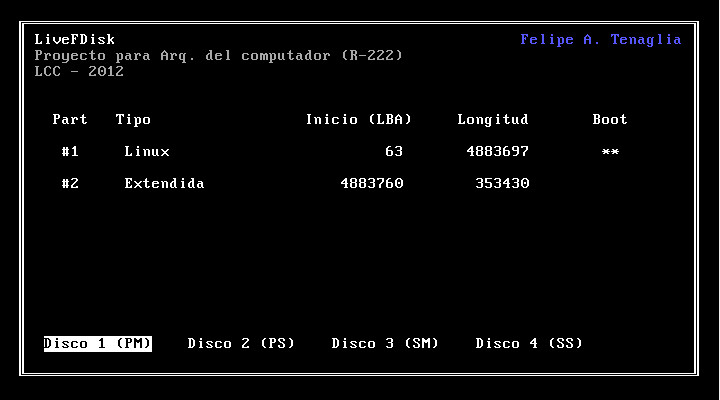
\includegraphics[width=1\textwidth]{Screenshot.jpg}
\caption{ Captura de pantalla del programa }
\label{fig:screenshot}
\end{figure}

\subsection*{Comandos del teclado} 
\begin{itemize}
\item \verb!1 - 4 = ! Cambia el disco activo (1 = Primary Master, 2 = Primary Slave, 3 = Secondary Master, 4 = Secondary Slave)
\item \verb!E = ! Habilita el men\'u para la eliminaci\'on de particiones
\item \verb!U = ! Alterna las unidades de visualizaci\'on (Ternas CHS o sectores)
\end{itemize}

\section*{Problemas y dificultades}
Durante el desarrollo me surgieron algunas dificultades, relacionadas tanto con decisiones de dise\~no, como tambi\'en con impedimentos propios de la BIOS.

\subsection*{L\'imite de bytes}
Como es sabido, para los \textit{bootloaders} existe un l\'imite de 512 bytes. \footnote{En la pr\'actica son 510 bytes ya que los ultimos 2 corresponden a la 'firma': 0x55AA} En un principio hab\'ia decidido dise\~nar el programa de manera \'optima para que el tama\~no de su binario no exceda este l\'imite, pero para poder agregarle funciones y para mejorar la interfaz de usuario, decid\'i separar al programa en 2 etapas.
\\

La primera etapa cumple con el l\'imite de 512 bytes y es la encargada de borrar la pantalla, leer el disco y cargar la segunda etapa. La segunda instancia es el programa considerado en s\'i mismo. En \'el, mediante las llamadas a la BIOS y a trav\'es de los puertos, podemos leer la tabla de particiones de los 4 discos principales, si estos existen.

\subsection*{Administraci\'on de memoria}

En parte relacionado con el apartado anterior, la administraci\'on de memoria fue un punto a considerar, ya que debiamos establecer para cada etapa, principalmente, donde estar\'ia alojado el c\'odigo y su respectivo \textit{stack} y en donde almacenar\'iamos el MBR le\'ido, todo esto considerando la limitaci\'on de memoria propia al estar ejecut\'andose el programa en \textit{modo real}. Finalmente el mapa de memoria qued\'o establecido como se ve en la Figura \ref{fig:memoria}.

\begin{figure}
\centering
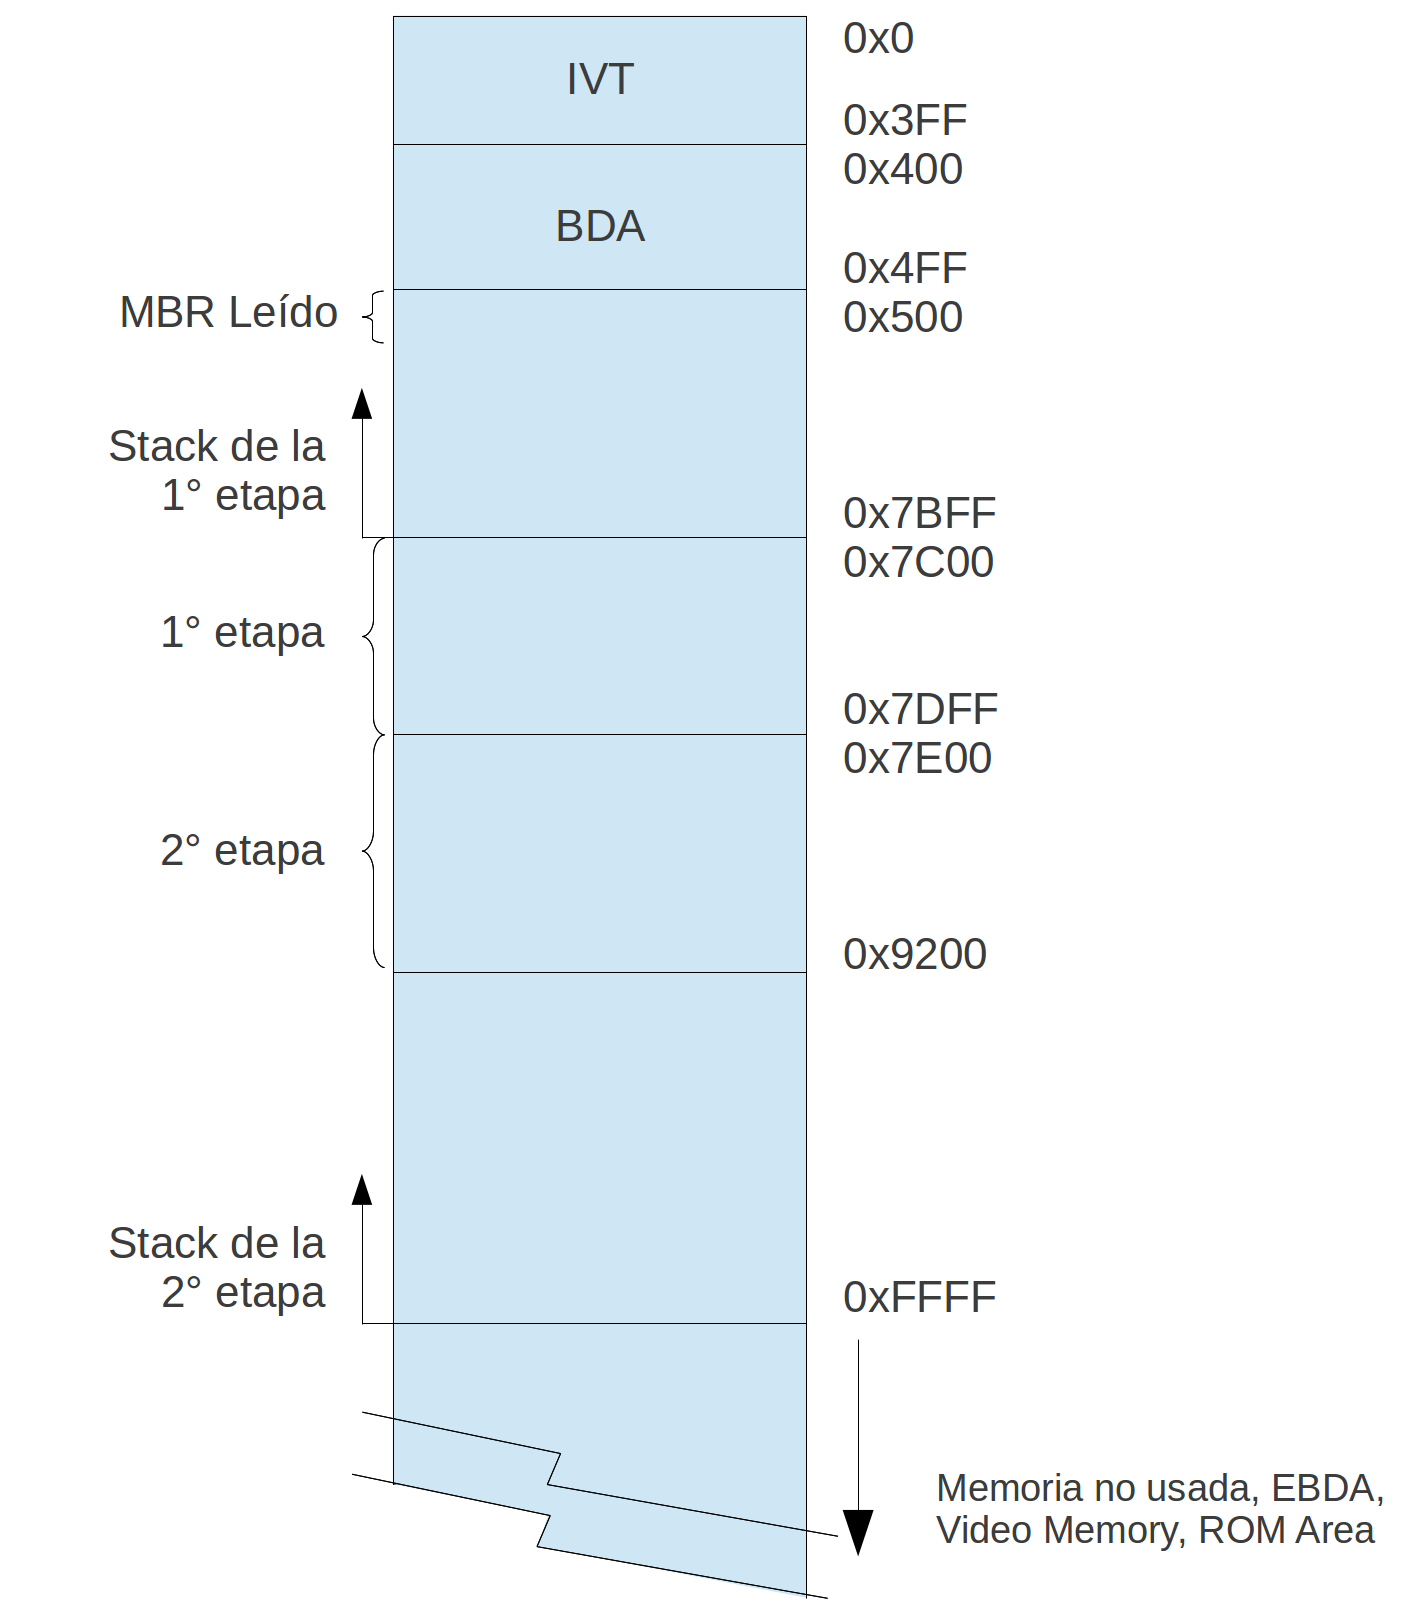
\includegraphics[scale=0.8]{Memoria.png}
\caption{ Mapa de memoria del programa }
\label{fig:memoria}
\end{figure}

\subsection*{Conflicto entre interrupciones}

Durante el desarrollo, al incorporar el manejo de los discos a trav\'es del teclado, por alguna raz\'on al ejecutar la interrupci\'on de acceso a disco (\verb!INT 0x13!) luego de una interrupci\'on de teclado (\verb!INT 0x16!), estas colisionaban, bloqueando el acceso a disco a trav\'es de esta interrupci\'on, por lo tanto decid\'i que la lectura del MBR se realice directamente a trav\'es de puertos.

\section*{Multiboot Specification}
Para lograr generar un kernel que pueda ser booteado con alg\'un gestor de arranque compatible con la Multiboot Specification (i.e. GRUB), le\'i la especificaci\'on e inclu\'i el header como se explica en ella.
\\

Adem\'as hubo que cambiar las interrupciones de BIOS por lectura y escritura de puertos, ya que por estar ejecut\'andose nuestro programa en modo protegido, estas no son soportadas.

\section*{Posibles extensiones}

Como fue propuesto se puede extender para que se puedan crear y modificar las particiones primarias como as\'i tambi\'en incluir la opci\'on de formatear dichas particiones. Tambi\'en se podr\'ia incorporar la capacidad de listar las particiones l\'ogicas.
\\

Una extensi\'on m\'as simple puede ser mejorarle el reconocimiento de tipos de particiones, ya que actualmente est\'a limitado a:
\begin{itemize}
\item Extendida (\verb!0x5!)
\item FAT16 (\verb!0x6!)
\item NTFS (\verb!0x7!)
\item FAT32 (\verb!0xB!)
\item Linux Swap (\verb!0x82!)
\item Linux (\verb!0x83!)
\end{itemize}

\section*{Referencias}
\begin{itemize}
\item \htmladdnormallink {Documentación de NASM}{http://www.nasm.us/doc/nasmdoc0.html}
\item \htmladdnormallink {Wikipedia: MBR}{http://es.wikipedia.org/wiki/MBR}
\item \htmladdnormallink {OSDev.org}{http://wiki.osdev.org/Main_Page}
\item \htmladdnormallink {MultiBoot Specification}{http://www.gnu.org/software/grub/manual/multiboot/multiboot.html}
\end{itemize}

\end{document}
